%%%%%%%%%%%%%%%%%%%%%%%%%%%%%%%%%%%%%%%%%%%%%%%%%%%%%%%%%%%%%%%%%%%%%%%%%%%%%%%%%%
\begin{frame}[fragile]\frametitle{}
\begin{center}
{\Large Conclusions}
\end{center}
\end{frame}

%%%%%%%%%%%%%%%%%%%%%%%%%%%%%%%%%%%%%%%%%%%%%%%%%%%%%%%%%%%
\begin{frame}[fragile]\frametitle{One pager}

\begin{itemize}
\item \textbf{Models:} Building blocks supporting different AI model types - LLMs, Chat, Text Embeddings.
\item \textbf{Prompts:} Inputs constructed from various components. LangChain offers easy interfaces - Prompt Templates, Example Selectors, Output Parsers.
\item \textbf{Memory:} Stores/retrieves messages, short or long term, in conversations.
\item \textbf{Indexes:} Assist LLMs with documents - Document Loaders, Text Splitters, Vector Stores, Retrievers.
\item \textbf{Chains:} Combine components or chains in order to accomplish tasks.
\item \textbf{Agents:} Empower LLMs to interact with external systems, make decisions, and complete tasks using Tools.
\end{itemize}

\begin{center}
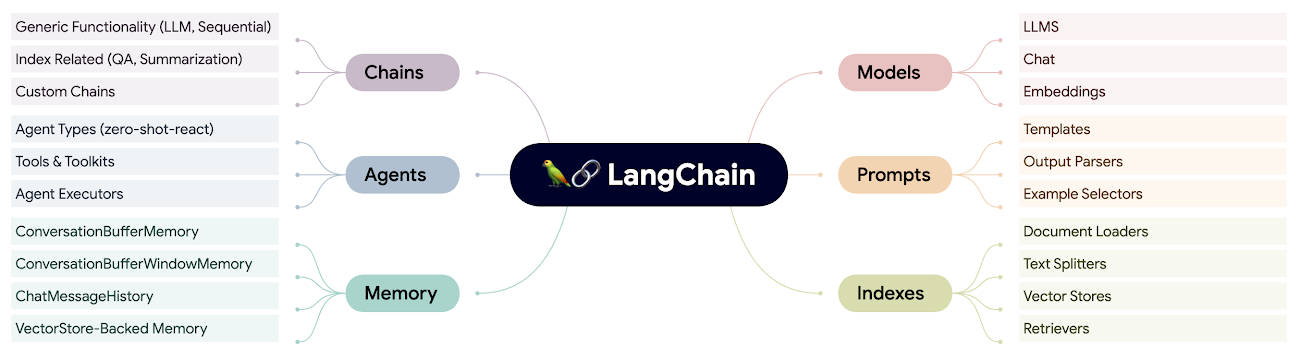
\includegraphics[width=0.8\linewidth,keepaspectratio]{llm99}
\end{center}


{\tiny (Ref: Building Generative AI applications made easy with Vertex AI PaLM API and LangChain  - Anand Iyer, Rajesh Thallam)}

\end{frame}


%%%%%%%%%%%%%%%%%%%%%%%%%%%%%%%%%%%%%%%%%%%%%%%%%%%%%%%%%%%
\begin{frame}[fragile]\frametitle{Closing Thoughts}

\begin{itemize}
\item Langchain's usefulness in solving problems today
\item Possibility of LLM APIs expanding capabilities over time
\item Potential for Langchain to become an interface to LLMs
\item Acknowledgment of Langchain's valuable contributions and community efforts
\item Appreciation for the work done by Harrison and the Langchain team
\end{itemize}

{\tiny (Ref: What is Langchain and why should I care as a developer? - Logan Kilpatrick)}

\end{frame}
